\section{Methods}
Our method models two types of signal from the data: (i) change of the allele distributions at SNP loci (discussed in Section \ref{ss:allele_distrib}), and (ii) change in number of fragments sequenced from a larger genomic region (discussed in Section \ref{ss:coverage}). Though each of these is noisy, the two are (nearly) independent (modulo number of reads overlapping the SNP position) variables and can be combined into a single generative model. For this purpose we use a Hidden Markov Model (HMM), where we interpret the allele counts at SNP loci as emissions, while the coverage is used as a prior probability for each state (see section \ref{ss:hmm}). 

For our method we assume that we have both Wholge Genome Sequencing (WGS) data for parents and deep sequencing data of cfDNA from maternal plasma. Both parental genomes are phased (based on 1000 Genomes data, see Section \ref{data}). All \textit{de novo} CNVs thus correspond to a particular parental haplotype duplication or deletion event. Labelling the two maternal and paternal haplotypes as $M_A,M_B,P_A,P_B$. For each inheritance pattern (normal inheritance, maternal duplication, paternal duplication, maternal deletion, paternal deletion) we introduce a set of \textit{phased inheritance patterns} that enumerates all the possible configurations of fetal haplotypes corresponding to the respective inheritance pattern. For example a duplication in the maternal zygote (egg) will consist of one (or more) 
of  six phased inheritance patterns: 
$$M_AM_AP_A, M_AM_BP_A, M_BM_BP_A, M_AM_AP_B, M_AM_BP_B, M_BM_BP_B$$
There are a total of 20 phased inheritance pattern ($PP$): 6 each for maternal/paternal duplication, 2 each for maternal/paternal deletion, and 4 for normal inharitance). We refer to the number of alleles inherited by the fetus as $|PP|$. We use $r$ to refer to the percentage of cfDNA that is fetus-derived; this parameter is estimated from positions in the genome where the parents are homozygous for alternate alleles.


\subsection{SNP Allele Distribution}\label{ss:allele_distrib}
For every SNP locus we observe a distribution of nucleotides in maternal plasma reads. In this section we focus on calculating the probability of the observation with respect to a phased inheritance pattern. Formally, we observe the counts of the 4  nucleotides $\{k_\A, k_\C, k_\G, k_\T\}$ and compute the probability of observing each of these from a particular phased inheritance pattern $\PP$ based on the  Poisson distribution, approximated by a Gaussian, i.e.
\begin{align}
Pr[\(k_x\) ~|~  M_A, M_B; P_A, P_B; r; \PP] \sim \N\(\mu_x, \mu_x\)
\end{align}
To compute $\mu_x, x \in \{\A,\C,\G,\T\}$, we first adjust the mixture ratio $r$  based on the expected number of fetal haplotypes $|PP|$. 
\begin{align}
r' =&  \frac{ |PP| \cdot r/2 }{|PP| \cdot r/2 ~+~ (1-r) }
\end{align}
Then for each nucleotide $x$ we sum probabilities of all the possible sources it might have been sequenced from, which includes maternal haplotypes and fetal haplotypes:
\begin{align}
p_x &= \sum_{i = A}^B [x \text{ equals } M_i] \cdot m_i (1-r')/2  \\
	&~~~ + \sum_{i = 1}^{|PP|} [x \in PP] \cdot r'/|PP|  \nonumber
\end{align}
For reads putatively coming from indigenous maternal DNA, we correct for maternal CNVs by using the allele ratios $m_i$ as observed in maternal-only sequencing data. Additionally, in order to mitigate noise we add pseudocount $\alpha$ (proportional to the genome-wide coverage) to these counts.
\begin{align}
m_i &= \frac{\alpha + \# \text{reads supporting }M_i\text{ in maternal seqencing}}{2\alpha + \sum_{j=A}^{B}\# \text{reads supporting }M_j\text{ in maternal seqencing}}
\end{align}
We thus obtain the expected probability distribution for each nucleotide observed at this SNP locus.  To get the expected number of reads supporting particular variant at this SNP locus, we have to multiply $p_x$ by the number of reads mapped,
\begin{align}
\mu_x &= p_x \cdot \#\text{mapped reads}
\end{align}
As we describe lower, we use this probability distribution $\N\(\mu, \mu \)$ that is conditional on phased pattern $\PP$ as the emission distribution for each nucleotide in our HMM.

\subsection{CNVs and Depth of Coverage}\label{ss:coverage}
Variations in number of fragments sequenced per a region is a standard measure used for detection of mid to large sized CNVs (see \cite{medvedev2009} for a review), and has lately been used for CNV detection from maternal plasma \cite{srinivasan2013, chen2013} as well. However the relatively low admixture of fetal DNA in the maternal plasma together with cfDNA sequencing biases considerably limit potential of methods relying on coverage signal from a single sample. Furthermore, the high variability of the coverage derived from blood plasma (Figure \ref{fig:fpkm}A) makes it difficult to identify shorter CNVs .Thus methods \cite{srinivasan2013, chen2013} require multiple datasets to establish a baseline for CNV calling.

Simultaneously, the coverage forms an important \textbf{complimentary} signal to the allelic distributions described above: certain ratios have very similar probability under different phased patterns, e.g. a deletion of a maternally inherited allele may yield distributions similar to a paternally inherited duplication. Incorporating the coverage signal helps to discriminate such states. In our method, we use the coverage information as a noisy predictor to complement the signal we obtain from SNP loci. For a reference plasma sequencing coverage we use plasma sample of the G1 trio of \cite{kitzman2012} dataset, as the overall coverages observed in large bins between the two samples correlate well ($R^2$=0.71; see Figure \ref{fig:fpkm}B). Availability of additional plasma datasets would enable us to further improve the accuracy of the reference bins.

First, for each SNP $i$ we compute \emph{window ratio value} $\WRV_i$ for a window $W_i$ of size 1Kb centred to the $i$-th SNP. This measure is analogous to the \emph{bin ratio value} in \cite{srinivasan2013}, and we compute it as a ratio of number of fragments $N_{W_i}$ mapped to $W_i$ to sum of fragments mapped to 200 1Kb windows with $\G\C$ content closest to $W_i$
\begin{align}
\WRV_i &= \frac{ N_{W_i} }{ \mathlarger{\sum_{W \in neigh_{\G\C}^{200}(W_i)}} N_{W} }
\end{align}
Window ratio values are independent of $\G\C$ content and depth of sequencing, thus for a particular window they are directly comparable between different samples. We model the difference between $\WRV_i^S$ in the studied plasma sample and $\WRV_i^R$ in the reference plasma sample as a Gaussian noise with zero mean and empirically estimated variance $\sigma_{\text{noise}}$. 

We then estimate the probability of the observed number of fragments $N_{W_i}$ in $W_i$ conditional on number of fetal haplotypes ($|PP|$), which is either three for duplication, one for deletion, or two for normal inheritance. Therefore we compute two more $\WRV_i^R$s, each scaled to reflect one CNV type. For duplication, we would expect to see $(1+r/2)$ times more fragments while for deletion $(1-r/2)$ times less fragments, thus the scaled $\WRV_i^{R,|PP|}$ is estimated as
\begin{align}
\WRV_i^{R,|PP|} = \frac{ N_{W_i^R} \cdot (1+(|PP|\-2)\cdot r/2) }{ \mathlarger{\sum_{W \in neigh_{\G\C}^{200}(W_i^R)}} N_{W^R} }
\end{align}

Note that compared to previous methods we use significantly smaller windows: 1kb versus 100kb-1Mb used previously \cite{chen2013, srinivasan2013}. As mentioned earlier, our goal here is not to detect CNVs immediately, but to rather compute a probability distribution over the number of haplotypes the fetus has inherited, which are used as  priors in the more complex model. Due to the independence assumptions inherent in the HMM we want these priors, applied at each state, to be (approximately) independent, and hence we pick a window size so that windows of adjacent SNPs are unlikely to overlap. We compute the probability of $\WRV_i^S$  being generated from an event fetal allele copy count $|PP|$ as $\N(\WRV_i^{R,|PP|}-\WRV_i^S; \mu=0, \sigma_{\text{noise}})$. We then normalize these to obtain priors for each phased pattern used in the HMM described in the next section. 

\begin{figure}[h]
%\missingfigure{The main HMM}
\subfigure[]{\label{fig:scatter:a}
\begin{minipage}[b]{0.45\textwidth}
		\centering
		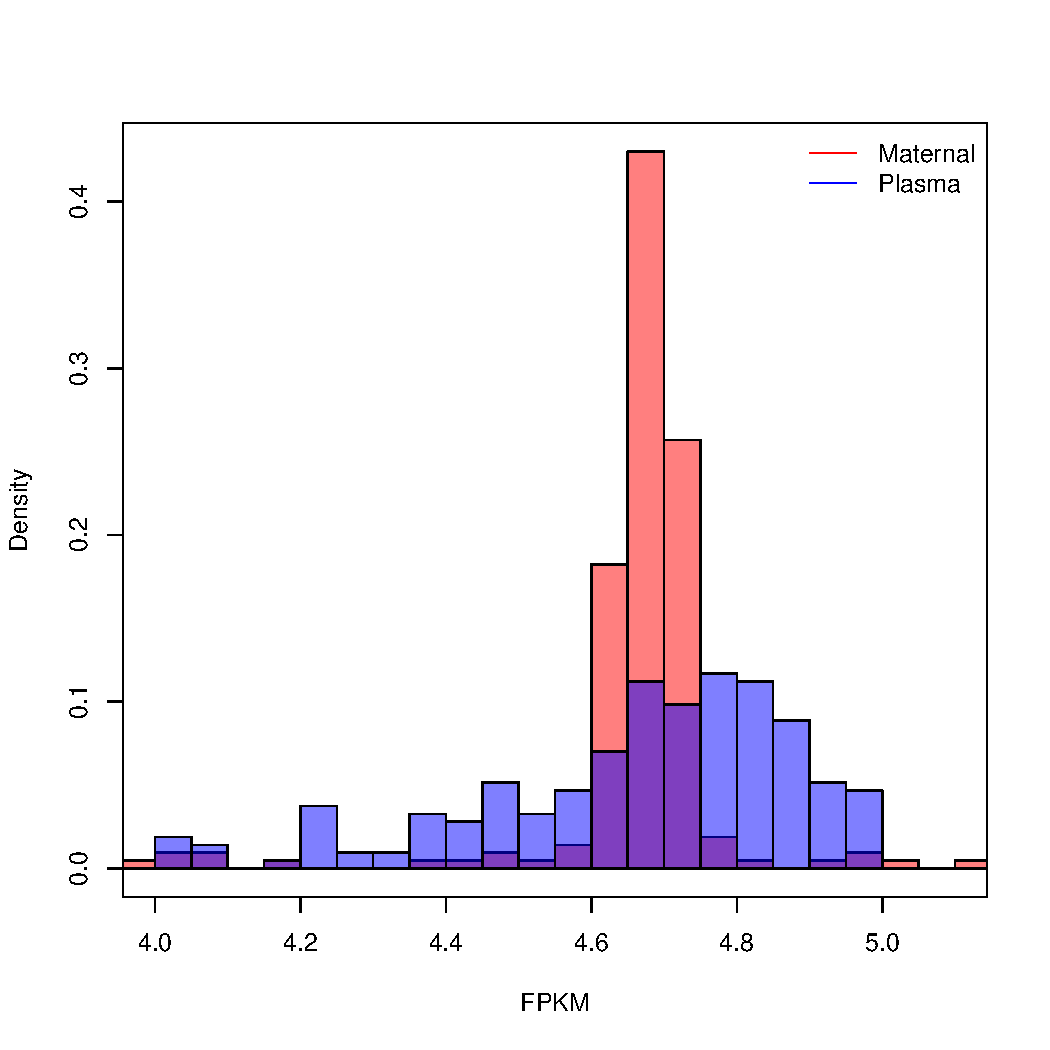
\includegraphics[height=0.35\textheight]{figures/histo}

		\end{minipage}	

}
\hspace{20pt}
\subfigure[]{\label{fig:histo:b}
	\begin{minipage}[b]{0.45\textwidth}
		\centering
	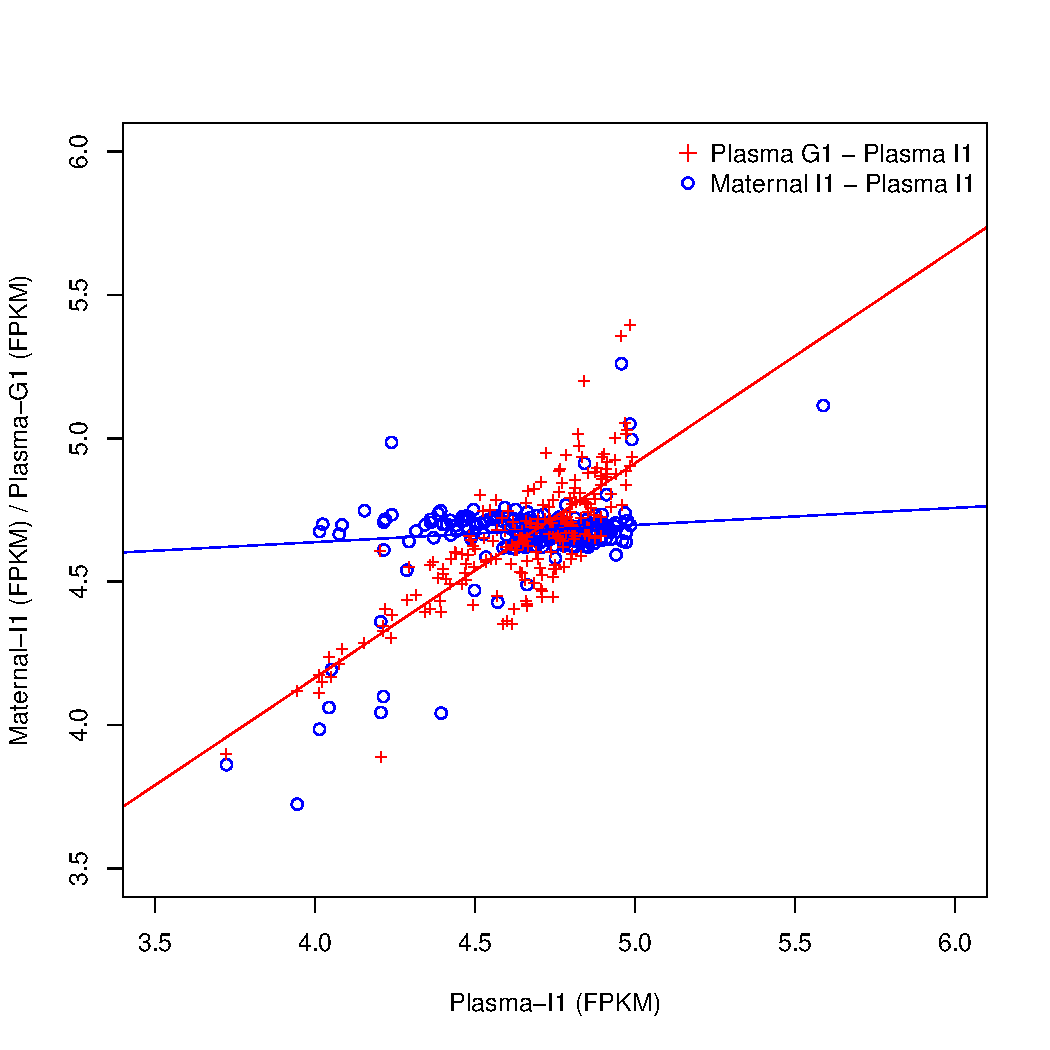
\includegraphics[height=0.35\textheight]{figures/scatter}

	\end{minipage}	
}
	
\label{fig:fpkm}
\caption{(a) Distribution of fragments per kilobase of chromosome 1 per million fragments (FPKM) in 1 megabase segments for plasma sample (blue) and maternal sample (red) of the I1 trio. (b) Scatterplot demonstrating the Correlation of FPKM between plasma samples of I1 and G1 trios (circles), and between I1 plasma sample and I1 maternal sample (crosses). The fit lines are estemiated by an iteratively reweighted least squares method. Coverage variaiton of cfDNA from plasma has much wider distribution than standard WGS. Thus sample from other plasma is more suitable than the same trio maternal sample for purpose of coverage distribution reference in our model.  }\label{fig:fpkm}
\end{figure}

\subsection{Hidden Markov Model for CNV Inference}\label{ss:hmm}
To combine the signals form individual SNP positions, we use an HMM with 20 states corresponding to modelled phased inheritance patterns (Figure \ref{fig:hmm_main}). States representing normal inheritance are central to the model assuming that two CNVs cannot be immediately subsequent. Between states of the same inheritance pattern, we allow for transitions reflecting either errors in phasing or recombinations. For each state, the emissions are the counts of individual alleles in reads mapped to that particular SNP position. The probability of the observed emission is the probability of such allele counts in the expected allele distribution conditional on phased inheritance pattern as described above in \ref{ss:allele_distrib}.

To incorporate the coverage information, for each SNP position we multiply the transition probabilities into the state by the copy number priors obtained in the previous section. Specifically, each edge incoming to a state is multiplied by the corresponding prior of inheriting that many haplotypes, which are then normalized so that the sum of the probabilities leaving each state is one. %the transition probabilities  \ref{fig:hmm_main:a}

The transition probabilities within an event type (e.g. maternal duplication) were set as $0.01$, to reflect expected haplotype block lengths of several hundred SNPs. Further, the transition probability for starting a CNV was set to one in ten thousand SNP loci ($0.0001$) with length expected to span approximately one thousand SNPs (transition probability back to normal inheritance was set to $0.001$).

\begin{figure}[h]
%\missingfigure{The main HMM}
\centering
\subfigure[Overall HMM architecture]{\label{fig:hmm_main:a}
	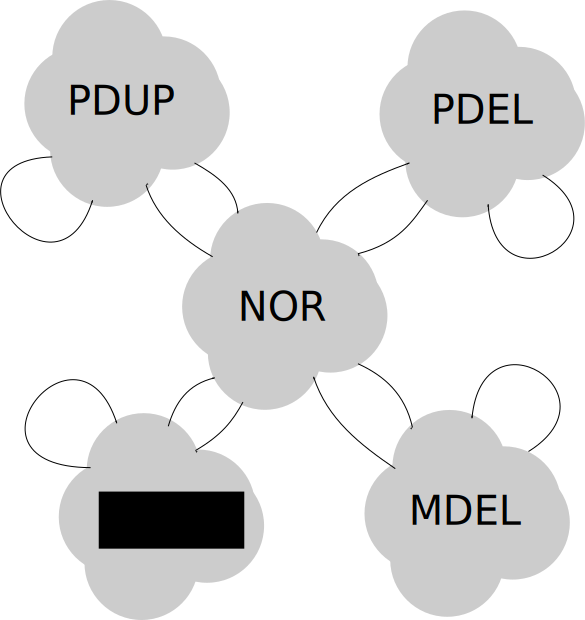
\includegraphics[height=0.2\textheight]{figures/main-HMM}
	\quad
}
\hspace{20pt}
\subfigure[States for normal inheritance]{
	\begin{minipage}[b]{0.45\textwidth}
		\centering
		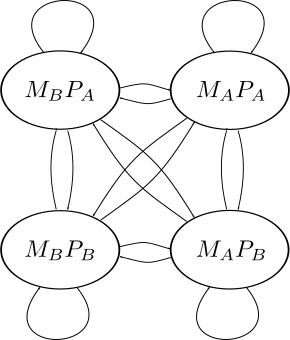
\includegraphics[height=0.2\textheight]{figures/NOR-HMM}
		\vspace{8pt}
	\end{minipage}	
}

\vspace{10pt}
\subfigure[States for maternal duplication]{
\begin{minipage}[b]{0.4\textwidth}
	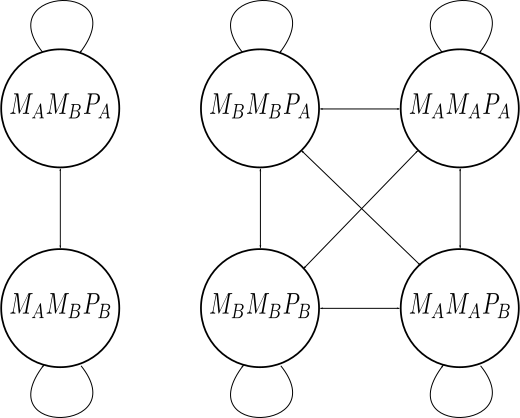
\includegraphics[height=0.2\textheight]{figures/DUP-HMM}
	\end{minipage}	
}
\hspace{0pt}
\subfigure[States for maternal deletion]{
	\begin{minipage}[b]{0.4\textwidth}
		\centering
		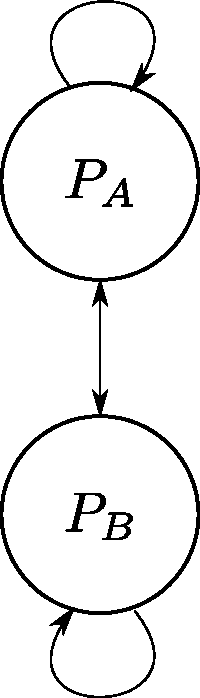
\includegraphics[height=0.2\textheight]{figures/DEL-HMM}
	\end{minipage}	
}

\caption{Hidden Markov model used for CNV inference. (a) High-level architecture of the HMM with 5 sets of states corresponding to 5 types of fetal inheritance. Note, we do not allow two CNVs to be adjacent, thus switching between two CNVs always has to go through normal inheritance state. Edges in (a) represent edges coming in/out of all states between two sets of states. (b-d) Correspond to the diagram of states of the HMM within the normal inheritance, maternal duplication, and maternal deletion states of (a). Paternal duplications/deletions are anaIogous to (c) and (d). Inner edges in (b-d) serve to model errors in phasing or recombination events.}\label{fig:hmm_main}
\end{figure}

\input simulation
